% Options for packages loaded elsewhere
\PassOptionsToPackage{unicode}{hyperref}
\PassOptionsToPackage{hyphens}{url}
%
\documentclass[
]{article}
\title{Amazing Document}
\author{Filippo Gambarota}
\date{Updated on 2022-03-07}

\usepackage{amsmath,amssymb}
\usepackage{lmodern}
\usepackage{iftex}
\ifPDFTeX
  \usepackage[T1]{fontenc}
  \usepackage[utf8]{inputenc}
  \usepackage{textcomp} % provide euro and other symbols
\else % if luatex or xetex
  \usepackage{unicode-math}
  \defaultfontfeatures{Scale=MatchLowercase}
  \defaultfontfeatures[\rmfamily]{Ligatures=TeX,Scale=1}
\fi
% Use upquote if available, for straight quotes in verbatim environments
\IfFileExists{upquote.sty}{\usepackage{upquote}}{}
\IfFileExists{microtype.sty}{% use microtype if available
  \usepackage[]{microtype}
  \UseMicrotypeSet[protrusion]{basicmath} % disable protrusion for tt fonts
}{}
\makeatletter
\@ifundefined{KOMAClassName}{% if non-KOMA class
  \IfFileExists{parskip.sty}{%
    \usepackage{parskip}
  }{% else
    \setlength{\parindent}{0pt}
    \setlength{\parskip}{6pt plus 2pt minus 1pt}}
}{% if KOMA class
  \KOMAoptions{parskip=half}}
\makeatother
\usepackage{xcolor}
\IfFileExists{xurl.sty}{\usepackage{xurl}}{} % add URL line breaks if available
\IfFileExists{bookmark.sty}{\usepackage{bookmark}}{\usepackage{hyperref}}
\hypersetup{
  pdftitle={Amazing Document},
  pdfauthor={Filippo Gambarota},
  hidelinks,
  pdfcreator={LaTeX via pandoc}}
\urlstyle{same} % disable monospaced font for URLs
\usepackage[margin=1in]{geometry}
\usepackage{color}
\usepackage{fancyvrb}
\newcommand{\VerbBar}{|}
\newcommand{\VERB}{\Verb[commandchars=\\\{\}]}
\DefineVerbatimEnvironment{Highlighting}{Verbatim}{commandchars=\\\{\}}
% Add ',fontsize=\small' for more characters per line
\usepackage{framed}
\definecolor{shadecolor}{RGB}{248,248,248}
\newenvironment{Shaded}{\begin{snugshade}}{\end{snugshade}}
\newcommand{\AlertTok}[1]{\textcolor[rgb]{0.94,0.16,0.16}{#1}}
\newcommand{\AnnotationTok}[1]{\textcolor[rgb]{0.56,0.35,0.01}{\textbf{\textit{#1}}}}
\newcommand{\AttributeTok}[1]{\textcolor[rgb]{0.77,0.63,0.00}{#1}}
\newcommand{\BaseNTok}[1]{\textcolor[rgb]{0.00,0.00,0.81}{#1}}
\newcommand{\BuiltInTok}[1]{#1}
\newcommand{\CharTok}[1]{\textcolor[rgb]{0.31,0.60,0.02}{#1}}
\newcommand{\CommentTok}[1]{\textcolor[rgb]{0.56,0.35,0.01}{\textit{#1}}}
\newcommand{\CommentVarTok}[1]{\textcolor[rgb]{0.56,0.35,0.01}{\textbf{\textit{#1}}}}
\newcommand{\ConstantTok}[1]{\textcolor[rgb]{0.00,0.00,0.00}{#1}}
\newcommand{\ControlFlowTok}[1]{\textcolor[rgb]{0.13,0.29,0.53}{\textbf{#1}}}
\newcommand{\DataTypeTok}[1]{\textcolor[rgb]{0.13,0.29,0.53}{#1}}
\newcommand{\DecValTok}[1]{\textcolor[rgb]{0.00,0.00,0.81}{#1}}
\newcommand{\DocumentationTok}[1]{\textcolor[rgb]{0.56,0.35,0.01}{\textbf{\textit{#1}}}}
\newcommand{\ErrorTok}[1]{\textcolor[rgb]{0.64,0.00,0.00}{\textbf{#1}}}
\newcommand{\ExtensionTok}[1]{#1}
\newcommand{\FloatTok}[1]{\textcolor[rgb]{0.00,0.00,0.81}{#1}}
\newcommand{\FunctionTok}[1]{\textcolor[rgb]{0.00,0.00,0.00}{#1}}
\newcommand{\ImportTok}[1]{#1}
\newcommand{\InformationTok}[1]{\textcolor[rgb]{0.56,0.35,0.01}{\textbf{\textit{#1}}}}
\newcommand{\KeywordTok}[1]{\textcolor[rgb]{0.13,0.29,0.53}{\textbf{#1}}}
\newcommand{\NormalTok}[1]{#1}
\newcommand{\OperatorTok}[1]{\textcolor[rgb]{0.81,0.36,0.00}{\textbf{#1}}}
\newcommand{\OtherTok}[1]{\textcolor[rgb]{0.56,0.35,0.01}{#1}}
\newcommand{\PreprocessorTok}[1]{\textcolor[rgb]{0.56,0.35,0.01}{\textit{#1}}}
\newcommand{\RegionMarkerTok}[1]{#1}
\newcommand{\SpecialCharTok}[1]{\textcolor[rgb]{0.00,0.00,0.00}{#1}}
\newcommand{\SpecialStringTok}[1]{\textcolor[rgb]{0.31,0.60,0.02}{#1}}
\newcommand{\StringTok}[1]{\textcolor[rgb]{0.31,0.60,0.02}{#1}}
\newcommand{\VariableTok}[1]{\textcolor[rgb]{0.00,0.00,0.00}{#1}}
\newcommand{\VerbatimStringTok}[1]{\textcolor[rgb]{0.31,0.60,0.02}{#1}}
\newcommand{\WarningTok}[1]{\textcolor[rgb]{0.56,0.35,0.01}{\textbf{\textit{#1}}}}
\usepackage{longtable,booktabs,array}
\usepackage{calc} % for calculating minipage widths
% Correct order of tables after \paragraph or \subparagraph
\usepackage{etoolbox}
\makeatletter
\patchcmd\longtable{\par}{\if@noskipsec\mbox{}\fi\par}{}{}
\makeatother
% Allow footnotes in longtable head/foot
\IfFileExists{footnotehyper.sty}{\usepackage{footnotehyper}}{\usepackage{footnote}}
\makesavenoteenv{longtable}
\usepackage{graphicx}
\makeatletter
\def\maxwidth{\ifdim\Gin@nat@width>\linewidth\linewidth\else\Gin@nat@width\fi}
\def\maxheight{\ifdim\Gin@nat@height>\textheight\textheight\else\Gin@nat@height\fi}
\makeatother
% Scale images if necessary, so that they will not overflow the page
% margins by default, and it is still possible to overwrite the defaults
% using explicit options in \includegraphics[width, height, ...]{}
\setkeys{Gin}{width=\maxwidth,height=\maxheight,keepaspectratio}
% Set default figure placement to htbp
\makeatletter
\def\fps@figure{htbp}
\makeatother
\usepackage[normalem]{ulem}
% Avoid problems with \sout in headers with hyperref
\pdfstringdefDisableCommands{\renewcommand{\sout}{}}
\setlength{\emergencystretch}{3em} % prevent overfull lines
\providecommand{\tightlist}{%
  \setlength{\itemsep}{0pt}\setlength{\parskip}{0pt}}
\setcounter{secnumdepth}{5}
\newlength{\cslhangindent}
\setlength{\cslhangindent}{1.5em}
\newlength{\csllabelwidth}
\setlength{\csllabelwidth}{3em}
\newlength{\cslentryspacingunit} % times entry-spacing
\setlength{\cslentryspacingunit}{\parskip}
\newenvironment{CSLReferences}[2] % #1 hanging-ident, #2 entry spacing
 {% don't indent paragraphs
  \setlength{\parindent}{0pt}
  % turn on hanging indent if param 1 is 1
  \ifodd #1
  \let\oldpar\par
  \def\par{\hangindent=\cslhangindent\oldpar}
  \fi
  % set entry spacing
  \setlength{\parskip}{#2\cslentryspacingunit}
 }%
 {}
\usepackage{calc}
\newcommand{\CSLBlock}[1]{#1\hfill\break}
\newcommand{\CSLLeftMargin}[1]{\parbox[t]{\csllabelwidth}{#1}}
\newcommand{\CSLRightInline}[1]{\parbox[t]{\linewidth - \csllabelwidth}{#1}\break}
\newcommand{\CSLIndent}[1]{\hspace{\cslhangindent}#1}
\usepackage{booktabs}
\usepackage{longtable}
\usepackage{array}
\usepackage{multirow}
\usepackage{wrapfig}
\usepackage{float}
\usepackage{colortbl}
\usepackage{pdflscape}
\usepackage{tabu}
\usepackage{threeparttable}
\usepackage{threeparttablex}
\usepackage[normalem]{ulem}
\usepackage{makecell}
\usepackage{xcolor}
\ifLuaTeX
  \usepackage{selnolig}  % disable illegal ligatures
\fi

\begin{document}
\maketitle

{
\setcounter{tocdepth}{2}
\tableofcontents
}
\listoffigures
\listoftables
\begin{Shaded}
\begin{Highlighting}[]
\FunctionTok{library}\NormalTok{(magrittr)}
\FunctionTok{library}\NormalTok{(kableExtra)}
\end{Highlighting}
\end{Shaded}

\begin{Shaded}
\begin{Highlighting}[]
\CommentTok{\# Qui definiamo delle funzioni che possono essere utili globalmente}

\NormalTok{mean\_sd }\OtherTok{\textless{}{-}} \ControlFlowTok{function}\NormalTok{(x)\{}
  \FunctionTok{sprintf}\NormalTok{(}\StringTok{"(M = \%s, SD = \%s)"}\NormalTok{,}
          \FunctionTok{round}\NormalTok{(}\FunctionTok{mean}\NormalTok{(x), }\DecValTok{2}\NormalTok{),}
          \FunctionTok{round}\NormalTok{(}\FunctionTok{sd}\NormalTok{(x), }\DecValTok{2}\NormalTok{))}
\NormalTok{\}}
\end{Highlighting}
\end{Shaded}

\hypertarget{bookdown}{%
\section{Bookdown}\label{bookdown}}

Questo file ha esattamente lo stesso contenuto del file \texttt{example-document} ma viene compilato in un formato leggermente diverso usando il pacchetto \href{https://bookdown.org/yihui/bookdown/}{\texttt{bookdown}}. Sebbene sia pensato per produrre libri, bookdown è utilissimi per documenti di una certa complessità come le tesi (capitoli, sezioni etc.). Infatti rispetto a documenti standard ci sono diverse funzioni come:

\begin{itemize}
\tightlist
\item
  hyperlink a figure e sezioni: quando volete dire ``come rappresentato in Fig. 4'' potete inserire automaticamente il link alla figura 4. Lo stesso per sezioni e tabelle.
\item
  Struttura più complessa: è possibile dividere il documento in capitoli, lavorare separatamente ai vari capitoli e poi unirli insieme in modo automatico mantenendo tutto collegato
\end{itemize}

\hypertarget{cross-reference}{%
\subsection{Cross-reference}\label{cross-reference}}

In Markdown creiamo una sezione con \texttt{\#\ sezione} o una sottosezione con \texttt{\#\#\ sottosezione}. Se inseriamo anche \texttt{\{label\}} possiamo associare ad una sezione un'etichetta da poter utilizzare ovunque. Ad esempio posso richiamare la sezione bookdown usando \texttt{\textbackslash{}@ref(bookdown)}. Ad esempio come indicato nella sezione\ref{bookdown}.

Lo stesso funziona anche con immagini e tabelle. In questo caso è importante assegnare un nome al chunk che produce la figura o la tabella e usare sempre \texttt{\textbackslash{}@ref(fig:label)}. Ad esempio richiamiamo la figura del nostro gatto con label \texttt{keycat}. Come mostrato in Fig. @fig(fig:keycat).

Per le tabelle invece è necessario che queste abbiano una caption e come per le figure un label nel chunk. Il problema delle tabelle è che i diversi pacchetti gestiscono le caption in modo diverso e quindi dovete capire come inserire una caption. Per il pacchetto \texttt{stargazer} ad esempio c'è questa soluzione \url{https://stackoverflow.com/a/58002110}.
Come mostrato in Tabella \texttt{\textbackslash{}@ref(tab:model)} \ref{tab:model}\ldots{}
Con \texttt{kableExtra} è molto più semplice gestire la caption essendo che è disponibile un argomento \texttt{caption} all'interno della funzione \texttt{kable(caption\ =\ "Dataset")}. A quel punto usiamo sempre \texttt{\textbackslash{}@ref(tab:label)} per chiamare la Tabella \ref{tab:tab-data}.

\hypertarget{sintassi-markdown}{%
\section{Sintassi Markdown}\label{sintassi-markdown}}

Abbiamo visto che la sintassi Mardown è molto semplice e leggibile. Possiamo mettere in \textbf{grassetto}, \emph{corsivo} ed anche \sout{barrare} una parola.

Gli spazi tra le parole non vengono intepretati come in Word, infatti possiamo mettere quanti spazi vogliamo (visibile solo nel file \texttt{.Rmd}) ma il risultato sarà sempre lo stesso.

Per fare un nuovo paragrafo (a capo con uno spazio) dobbiamo inserire una linea vuota tra una porzione di testo e l'altra.

\begin{verbatim}
... e con questo finiamo il primo paragrafo.

In questo modo possiamo avere un nuovo paragrafo. 
Se non mettiamo la linea bianca il testo continuerà sulla stessa riga.
\end{verbatim}

Se vogliamo inserire una porzione di codice, senza eseguirlo ma solo per distinguerlo dal testo possiamo racchiudere il testo tra 3 backticks:

\begin{verbatim}
print("Hello World!")
\end{verbatim}

Se vogliamo possiamo anche specificare il linguaggio del codice in modo da evidenziare le parti principali:

\begin{Shaded}
\begin{Highlighting}[]
\NormalTok{x }\OperatorTok{=} \DecValTok{1}\NormalTok{:}\DecValTok{10}
\BuiltInTok{print}\NormalTok{(x)}
\end{Highlighting}
\end{Shaded}

Possiamo anche usare il codice inline usando 2 backtics per differenziare una porzione di \texttt{codice} direttamente nel testo.

Possiamo inserire delle footnotes usando la sintassi \texttt{\^{}{[}testo{]}} dove \texttt{testo} è il contenuto della footnote. Questo è comodo perchè la scriviamo direttamente nel testo e non alla fine della pagina\footnote{Questa è la mia footnote}.

In generale, possiamo usare tutta la sintassi Markdown, e ci sono moltissime guide per impararla.

\hypertarget{sintassi-r-markdown}{%
\section{Sintassi R Markdown}\label{sintassi-r-markdown}}

Essendo R Markdown l'implementazione del linguaggio R, la sintassi per alcune operazioni è leggermente diversa da quella markdown. Per esempio il blocco di codice:

\begin{Shaded}
\begin{Highlighting}[]
\NormalTok{x }\OtherTok{\textless{}{-}} \DecValTok{1}\SpecialCharTok{:}\DecValTok{10}
\FunctionTok{print}\NormalTok{(x)}
\end{Highlighting}
\end{Shaded}

E' un blocco di codice generico che non viene interpretato. Se usiamo la sintassi di R Markdown:

\begin{Shaded}
\begin{Highlighting}[]
\NormalTok{x }\OtherTok{\textless{}{-}} \DecValTok{1}\SpecialCharTok{:}\DecValTok{10}
\FunctionTok{print}\NormalTok{(x)}
\end{Highlighting}
\end{Shaded}

\begin{verbatim}
##  [1]  1  2  3  4  5  6  7  8  9 10
\end{verbatim}

Allora il codice viene anche eseguito e il risultato viene inserito direttamente nel documento.

Lo stesso vale per un grafico:

\begin{Shaded}
\begin{Highlighting}[]
\FunctionTok{plot}\NormalTok{(mtcars}\SpecialCharTok{$}\NormalTok{mpg, mtcars}\SpecialCharTok{$}\NormalTok{disp, }\AttributeTok{pch =} \DecValTok{19}\NormalTok{)}
\end{Highlighting}
\end{Shaded}

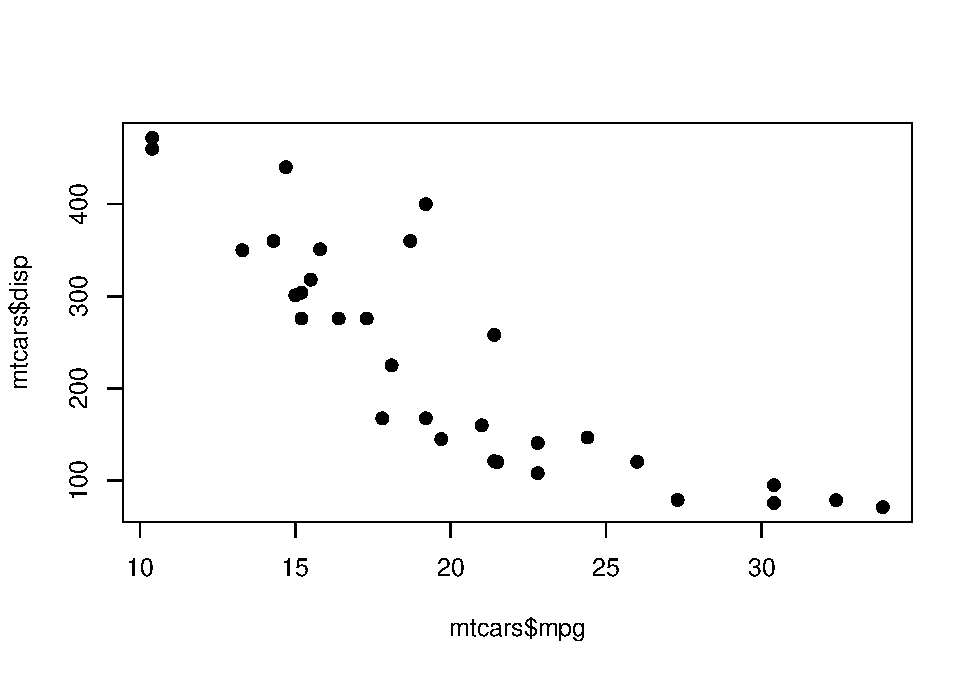
\includegraphics{example-bookdown_files/figure-latex/unnamed-chunk-2-1.pdf}

\hypertarget{immagini}{%
\section{Immagini}\label{immagini}}

Per le immagini possiamo usare due modalità principali:

\begin{itemize}
\tightlist
\item
  sintassi \texttt{markdown}: \texttt{!{[}caption{]}(file)}
\item
  sintassi \texttt{rmarkdown}: \texttt{knitr::include\_graphics(file)}
\end{itemize}

Il risultato è simile ma la seconda modalità è più semplice da personalizzare in termini di dimensioni, caption, etc.

\texttt{!{[}Word\ Meme{]}(img/word-meme.jpg)\{width=20\%\}}

\begin{figure}
\centering

\includegraphics[width=0.3\textwidth,height=\textheight]{img/word-meme.jpg}
\caption{Word Meme}
\end{figure}

\begin{Shaded}
\begin{Highlighting}[]
\NormalTok{knitr}\SpecialCharTok{::}\FunctionTok{include\_graphics}\NormalTok{(}\StringTok{"img/keyboard{-}cat.jpg"}\NormalTok{)}
\end{Highlighting}
\end{Shaded}

\begin{figure}

{\centering 
\includegraphics[width=0.3\linewidth]{img/keyboard-cat} 

}

\caption{Amazing Cat}\label{fig:keycat}
\end{figure}

\hypertarget{citazioni}{%
\section{Citazioni}\label{citazioni}}

Anche le citazioni sono facilissime da inserire. Quando citiamo nel testo vogliamo citare nel classico modo \texttt{(autore,\ anno)} oppure usare solo \texttt{(anno)} perchè citiamo il nome nel testo principale. Possiamo citare specificando il file \texttt{.bib} nello \texttt{YAML} e poi \texttt{{[}@key{]}}:

\begin{itemize}
\tightlist
\item
  citazione normale: (Xie et al., 2018)
\item
  citazione senza autore: (2018)
\item
  citazione multipla: (Vogel \& Machizawa, 2004; Xie et al., 2018)
\end{itemize}

Chiaramente se dovete cambiare lo stile (e.g., da APA a Chicago), sarà sufficiente cambiare il file \texttt{.csl} e ricompilare il documento. Le citazioni vengono poi inserite in automatico alla fine del documento.

\hypertarget{la-vera-potenza-di-r-markdown}{%
\section{La vera potenza di R Markdown}\label{la-vera-potenza-di-r-markdown}}

Il vero aspetto centrale di R Markdown è quello di poter automatizzare alcune operazioni che di solito sono tediose e con alta proababilità di errore. Ad esempio se dobbiamo riportare delle statistiche, solitamente dobbiamo scrivere manualmente i numeri, le parentesi, etc. Mentre se usiamo un documento R Markdown, codice, dati e testo sono tutti insieme. Facciamo un esempio:

Usiamo il dataset presente in R \texttt{mtcars} e immaginiamo sia il vostro dataset che dovere usare per la tesi o per il vostro report di analisi.

\begin{Shaded}
\begin{Highlighting}[]
\NormalTok{mtcars}
\end{Highlighting}
\end{Shaded}

\begin{verbatim}
##                      mpg cyl  disp  hp drat    wt  qsec vs am gear carb
## Mazda RX4           21.0   6 160.0 110 3.90 2.620 16.46  0  1    4    4
## Mazda RX4 Wag       21.0   6 160.0 110 3.90 2.875 17.02  0  1    4    4
## Datsun 710          22.8   4 108.0  93 3.85 2.320 18.61  1  1    4    1
## Hornet 4 Drive      21.4   6 258.0 110 3.08 3.215 19.44  1  0    3    1
## Hornet Sportabout   18.7   8 360.0 175 3.15 3.440 17.02  0  0    3    2
## Valiant             18.1   6 225.0 105 2.76 3.460 20.22  1  0    3    1
## Duster 360          14.3   8 360.0 245 3.21 3.570 15.84  0  0    3    4
## Merc 240D           24.4   4 146.7  62 3.69 3.190 20.00  1  0    4    2
## Merc 230            22.8   4 140.8  95 3.92 3.150 22.90  1  0    4    2
## Merc 280            19.2   6 167.6 123 3.92 3.440 18.30  1  0    4    4
## Merc 280C           17.8   6 167.6 123 3.92 3.440 18.90  1  0    4    4
## Merc 450SE          16.4   8 275.8 180 3.07 4.070 17.40  0  0    3    3
## Merc 450SL          17.3   8 275.8 180 3.07 3.730 17.60  0  0    3    3
## Merc 450SLC         15.2   8 275.8 180 3.07 3.780 18.00  0  0    3    3
## Cadillac Fleetwood  10.4   8 472.0 205 2.93 5.250 17.98  0  0    3    4
## Lincoln Continental 10.4   8 460.0 215 3.00 5.424 17.82  0  0    3    4
## Chrysler Imperial   14.7   8 440.0 230 3.23 5.345 17.42  0  0    3    4
## Fiat 128            32.4   4  78.7  66 4.08 2.200 19.47  1  1    4    1
## Honda Civic         30.4   4  75.7  52 4.93 1.615 18.52  1  1    4    2
## Toyota Corolla      33.9   4  71.1  65 4.22 1.835 19.90  1  1    4    1
## Toyota Corona       21.5   4 120.1  97 3.70 2.465 20.01  1  0    3    1
## Dodge Challenger    15.5   8 318.0 150 2.76 3.520 16.87  0  0    3    2
## AMC Javelin         15.2   8 304.0 150 3.15 3.435 17.30  0  0    3    2
## Camaro Z28          13.3   8 350.0 245 3.73 3.840 15.41  0  0    3    4
## Pontiac Firebird    19.2   8 400.0 175 3.08 3.845 17.05  0  0    3    2
## Fiat X1-9           27.3   4  79.0  66 4.08 1.935 18.90  1  1    4    1
## Porsche 914-2       26.0   4 120.3  91 4.43 2.140 16.70  0  1    5    2
## Lotus Europa        30.4   4  95.1 113 3.77 1.513 16.90  1  1    5    2
## Ford Pantera L      15.8   8 351.0 264 4.22 3.170 14.50  0  1    5    4
## Ferrari Dino        19.7   6 145.0 175 3.62 2.770 15.50  0  1    5    6
## Maserati Bora       15.0   8 301.0 335 3.54 3.570 14.60  0  1    5    8
## Volvo 142E          21.4   4 121.0 109 4.11 2.780 18.60  1  1    4    2
\end{verbatim}

Facciamo una tabella con il pacchetto \texttt{kableExtra}:

\begin{Shaded}
\begin{Highlighting}[]
\NormalTok{mtcars }\SpecialCharTok{\%\textgreater{}\%} 
  \FunctionTok{kable}\NormalTok{(}\AttributeTok{caption =} \StringTok{"Dataset"}\NormalTok{) }\SpecialCharTok{\%\textgreater{}\%} 
  \FunctionTok{kable\_styling}\NormalTok{()}
\end{Highlighting}
\end{Shaded}

\begin{table}

\caption{\label{tab:tab-data}Dataset}
\centering
\begin{tabular}[t]{l|r|r|r|r|r|r|r|r|r|r|r}
\hline
  & mpg & cyl & disp & hp & drat & wt & qsec & vs & am & gear & carb\\
\hline
Mazda RX4 & 21.0 & 6 & 160.0 & 110 & 3.90 & 2.620 & 16.46 & 0 & 1 & 4 & 4\\
\hline
Mazda RX4 Wag & 21.0 & 6 & 160.0 & 110 & 3.90 & 2.875 & 17.02 & 0 & 1 & 4 & 4\\
\hline
Datsun 710 & 22.8 & 4 & 108.0 & 93 & 3.85 & 2.320 & 18.61 & 1 & 1 & 4 & 1\\
\hline
Hornet 4 Drive & 21.4 & 6 & 258.0 & 110 & 3.08 & 3.215 & 19.44 & 1 & 0 & 3 & 1\\
\hline
Hornet Sportabout & 18.7 & 8 & 360.0 & 175 & 3.15 & 3.440 & 17.02 & 0 & 0 & 3 & 2\\
\hline
Valiant & 18.1 & 6 & 225.0 & 105 & 2.76 & 3.460 & 20.22 & 1 & 0 & 3 & 1\\
\hline
Duster 360 & 14.3 & 8 & 360.0 & 245 & 3.21 & 3.570 & 15.84 & 0 & 0 & 3 & 4\\
\hline
Merc 240D & 24.4 & 4 & 146.7 & 62 & 3.69 & 3.190 & 20.00 & 1 & 0 & 4 & 2\\
\hline
Merc 230 & 22.8 & 4 & 140.8 & 95 & 3.92 & 3.150 & 22.90 & 1 & 0 & 4 & 2\\
\hline
Merc 280 & 19.2 & 6 & 167.6 & 123 & 3.92 & 3.440 & 18.30 & 1 & 0 & 4 & 4\\
\hline
Merc 280C & 17.8 & 6 & 167.6 & 123 & 3.92 & 3.440 & 18.90 & 1 & 0 & 4 & 4\\
\hline
Merc 450SE & 16.4 & 8 & 275.8 & 180 & 3.07 & 4.070 & 17.40 & 0 & 0 & 3 & 3\\
\hline
Merc 450SL & 17.3 & 8 & 275.8 & 180 & 3.07 & 3.730 & 17.60 & 0 & 0 & 3 & 3\\
\hline
Merc 450SLC & 15.2 & 8 & 275.8 & 180 & 3.07 & 3.780 & 18.00 & 0 & 0 & 3 & 3\\
\hline
Cadillac Fleetwood & 10.4 & 8 & 472.0 & 205 & 2.93 & 5.250 & 17.98 & 0 & 0 & 3 & 4\\
\hline
Lincoln Continental & 10.4 & 8 & 460.0 & 215 & 3.00 & 5.424 & 17.82 & 0 & 0 & 3 & 4\\
\hline
Chrysler Imperial & 14.7 & 8 & 440.0 & 230 & 3.23 & 5.345 & 17.42 & 0 & 0 & 3 & 4\\
\hline
Fiat 128 & 32.4 & 4 & 78.7 & 66 & 4.08 & 2.200 & 19.47 & 1 & 1 & 4 & 1\\
\hline
Honda Civic & 30.4 & 4 & 75.7 & 52 & 4.93 & 1.615 & 18.52 & 1 & 1 & 4 & 2\\
\hline
Toyota Corolla & 33.9 & 4 & 71.1 & 65 & 4.22 & 1.835 & 19.90 & 1 & 1 & 4 & 1\\
\hline
Toyota Corona & 21.5 & 4 & 120.1 & 97 & 3.70 & 2.465 & 20.01 & 1 & 0 & 3 & 1\\
\hline
Dodge Challenger & 15.5 & 8 & 318.0 & 150 & 2.76 & 3.520 & 16.87 & 0 & 0 & 3 & 2\\
\hline
AMC Javelin & 15.2 & 8 & 304.0 & 150 & 3.15 & 3.435 & 17.30 & 0 & 0 & 3 & 2\\
\hline
Camaro Z28 & 13.3 & 8 & 350.0 & 245 & 3.73 & 3.840 & 15.41 & 0 & 0 & 3 & 4\\
\hline
Pontiac Firebird & 19.2 & 8 & 400.0 & 175 & 3.08 & 3.845 & 17.05 & 0 & 0 & 3 & 2\\
\hline
Fiat X1-9 & 27.3 & 4 & 79.0 & 66 & 4.08 & 1.935 & 18.90 & 1 & 1 & 4 & 1\\
\hline
Porsche 914-2 & 26.0 & 4 & 120.3 & 91 & 4.43 & 2.140 & 16.70 & 0 & 1 & 5 & 2\\
\hline
Lotus Europa & 30.4 & 4 & 95.1 & 113 & 3.77 & 1.513 & 16.90 & 1 & 1 & 5 & 2\\
\hline
Ford Pantera L & 15.8 & 8 & 351.0 & 264 & 4.22 & 3.170 & 14.50 & 0 & 1 & 5 & 4\\
\hline
Ferrari Dino & 19.7 & 6 & 145.0 & 175 & 3.62 & 2.770 & 15.50 & 0 & 1 & 5 & 6\\
\hline
Maserati Bora & 15.0 & 8 & 301.0 & 335 & 3.54 & 3.570 & 14.60 & 0 & 1 & 5 & 8\\
\hline
Volvo 142E & 21.4 & 4 & 121.0 & 109 & 4.11 & 2.780 & 18.60 & 1 & 1 & 4 & 2\\
\hline
\end{tabular}
\end{table}

Solitamente nel metodo di un articolo o di un report è necessario descrivere il dataset e riportare alcune statistiche descrittive. Con R Markdown posso usare dei code chunks (sia inline che come blocco) e usare delle funzioni R che producono del testo, senza scrivere direttamente i valori.

\begin{quote}
Ad esempio: Il dataset \texttt{mtcars} ha 32 osservazioni e 11 variabili. La variabile più importante è \texttt{mpg} (M = 20.09, SD = 6.03) (se state guardando il documento compilato guardate nel file \texttt{.Rmd} come i numeri vengono generati).
\end{quote}

Questo diventa ancora più rilevante se i dati in input cambiano. Se dobbiamo analizzare nuovamente i dati, cambiare delle parti o aggiornare, normalmente è necessario riscrivere tutto. In questo caso, semplicemente cambiando \texttt{mtcars} possiamo aggiornare tutto il testo che è legato ad \texttt{mtcars}:

\begin{Shaded}
\begin{Highlighting}[]
\CommentTok{\# aggiungo 10 righe a mtcars per simulare il fatto che i dati sono cambiati}
\NormalTok{mtcars }\OtherTok{\textless{}{-}} \FunctionTok{rbind}\NormalTok{(mtcars, mtcars[}\DecValTok{1}\SpecialCharTok{:}\DecValTok{10}\NormalTok{, ])}
\end{Highlighting}
\end{Shaded}

Ora ``eseguo'' nuovamente il codice di prima, come vedete (se state guardando il documento compilato guardate nel file \texttt{.Rmd} come i numeri vengono generati) tutto viene aggiornato senza cambiare nulla:

\begin{quote}
Ad esempio: Il dataset \texttt{mtcars} ha 42 osservazioni e 11 variabili. La variabile più importante è \texttt{mpg} (M = 20.16, SD = 5.42) (se state guardando il documento compilato guardate nel file \texttt{.Rmd} come i numeri vengono generati).
\end{quote}

\hypertarget{statistiche-piuxf9-complesse}{%
\subsection{Statistiche più complesse}\label{statistiche-piuxf9-complesse}}

Spesso dobbiamo creare tabelle da inserire nel nostro documento. Per esempio la tabella di un'analisi che abbiamo fatto. Fittiamo un modello di regressione lineare con il dataset \texttt{iris} e proviamo a predirre \texttt{Sepal.Length} con il fattore a 3 livelli \texttt{Species} (nota nel file \texttt{Rmd} come alcuni chunk vengono eseguiti in base all'output inserito):

\begin{Shaded}
\begin{Highlighting}[]
\NormalTok{fit }\OtherTok{\textless{}{-}} \FunctionTok{lm}\NormalTok{(Sepal.Length }\SpecialCharTok{\textasciitilde{}}\NormalTok{ Species, }\AttributeTok{data =}\NormalTok{ iris)}
\FunctionTok{summary}\NormalTok{(fit)}
\end{Highlighting}
\end{Shaded}

\begin{verbatim}
## 
## Call:
## lm(formula = Sepal.Length ~ Species, data = iris)
## 
## Residuals:
##     Min      1Q  Median      3Q     Max 
## -1.6880 -0.3285 -0.0060  0.3120  1.3120 
## 
## Coefficients:
##                   Estimate Std. Error t value Pr(>|t|)    
## (Intercept)         5.0060     0.0728  68.762  < 2e-16 ***
## Speciesversicolor   0.9300     0.1030   9.033 8.77e-16 ***
## Speciesvirginica    1.5820     0.1030  15.366  < 2e-16 ***
## ---
## Signif. codes:  0 '***' 0.001 '**' 0.01 '*' 0.05 '.' 0.1 ' ' 1
## 
## Residual standard error: 0.5148 on 147 degrees of freedom
## Multiple R-squared:  0.6187, Adjusted R-squared:  0.6135 
## F-statistic: 119.3 on 2 and 147 DF,  p-value: < 2.2e-16
\end{verbatim}

Ora vogliamo riportare tutti i valori (stime, confidence intervals e p-values) in una tabella. Possiamo crearla a mano, ma perchè non automatizzare il tutto. Ad esempio il pacchetto \texttt{sjPlot} ha diverse funzioni come \texttt{sjPlot::tab\_model()}:

Attenzione che non tutti gli output funzionano. Per esempio \texttt{sjPlot} funziona con documenti \texttt{html} mentre altri pacchetti (e.g., \texttt{stargazer}) funzionano con \texttt{pdf}:

\begin{Shaded}
\begin{Highlighting}[]
\NormalTok{stargazer}\SpecialCharTok{::}\FunctionTok{stargazer}\NormalTok{(fit, }\AttributeTok{header=}\ConstantTok{FALSE}\NormalTok{, }\AttributeTok{type=}\StringTok{\textquotesingle{}latex\textquotesingle{}}\NormalTok{, }\AttributeTok{title =} \StringTok{"(}\SpecialCharTok{\textbackslash{}\textbackslash{}}\StringTok{\#tab:model) Modello"}\NormalTok{)}
\end{Highlighting}
\end{Shaded}

\begin{table}[!htbp] \centering 
  \caption{\label{tab:model} Modello} 
  \label{} 
\begin{tabular}{@{\extracolsep{5pt}}lc} 
\\[-1.8ex]\hline 
\hline \\[-1.8ex] 
 & \multicolumn{1}{c}{\textit{Dependent variable:}} \\ 
\cline{2-2} 
\\[-1.8ex] & Sepal.Length \\ 
\hline \\[-1.8ex] 
 Speciesversicolor & 0.930$^{***}$ \\ 
  & (0.103) \\ 
  & \\ 
 Speciesvirginica & 1.582$^{***}$ \\ 
  & (0.103) \\ 
  & \\ 
 Constant & 5.006$^{***}$ \\ 
  & (0.073) \\ 
  & \\ 
\hline \\[-1.8ex] 
Observations & 150 \\ 
R$^{2}$ & 0.619 \\ 
Adjusted R$^{2}$ & 0.614 \\ 
Residual Std. Error & 0.515 (df = 147) \\ 
F Statistic & 119.265$^{***}$ (df = 2; 147) \\ 
\hline 
\hline \\[-1.8ex] 
\textit{Note:}  & \multicolumn{1}{r}{$^{*}$p$<$0.1; $^{**}$p$<$0.05; $^{***}$p$<$0.01} \\ 
\end{tabular} 
\end{table}

Possiamo anche creare un grafico direttamente dal modello usando il bellissimo pacchetto \texttt{effects}:

\begin{Shaded}
\begin{Highlighting}[]
\CommentTok{\# prende un modello e plotta gli effetti}
\FunctionTok{plot}\NormalTok{(effects}\SpecialCharTok{::}\FunctionTok{allEffects}\NormalTok{(fit)) }
\end{Highlighting}
\end{Shaded}

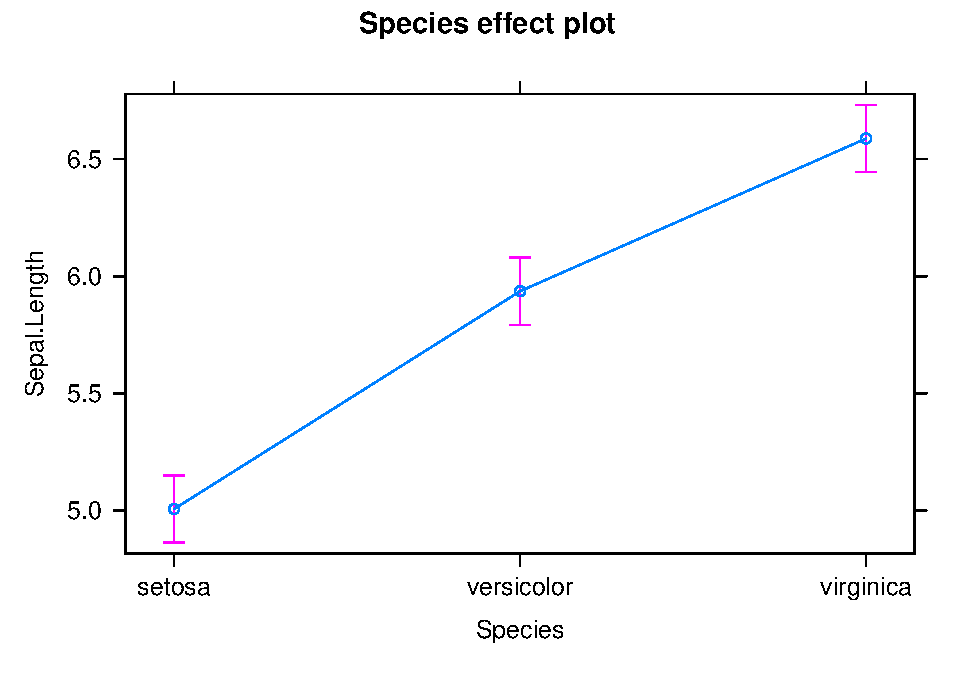
\includegraphics{example-bookdown_files/figure-latex/unnamed-chunk-8-1.pdf}

\hypertarget{bibliografia}{%
\section{Bibliografia}\label{bibliografia}}

\hypertarget{refs}{}
\begin{CSLReferences}{1}{0}
\leavevmode\vadjust pre{\hypertarget{ref-vogel2004}{}}%
Vogel, E. K., \& Machizawa, M. G. (2004). Neural activity predicts individual differences in visual working memory capacity. \emph{Nature}, \emph{428}(6984), 748--751.

\leavevmode\vadjust pre{\hypertarget{ref-xie2018r}{}}%
Xie, Y., Allaire, J. J., \& Grolemund, G. (2018). \emph{R markdown: The definitive guide}. Chapman; Hall/CRC.

\end{CSLReferences}

\end{document}
